%%%%%%%%%%%%%%%%%%%%%%%%%%%%%%%%%%%%%%%%%%%%%%%%%%%%%%%%%%%%%%%%%%%%%%%%%%%%%%%%
%2345678901234567890123456789012345678901234567890123456789012345678901234567890
%        1         2         3         4         5         6         7         8

\documentclass[letterpaper, 10 pt, conference]{ieeeconf}  % Comment this line out
                                                          % if you need a4paper
%\documentclass[a4paper, 10pt, conference]{ieeeconf}      % Use this line for a4
                                                          % paper

\IEEEoverridecommandlockouts                              % This command is only
                                                          % needed if you want to
                                                          % use the \thanks command
\overrideIEEEmargins
% See the \addtolength command later in the file to balance the column lengths
% on the last page of the document



% The following packages can be found on http:\\www.ctan.org
\usepackage{graphics} % for pdf, bitmapped graphics files
\usepackage{epsfig} % for postscript graphics files
\usepackage{mathptmx} % assumes new font selection scheme installed
\usepackage{times} % assumes new font selection scheme installed
\usepackage{amsmath} % assumes amsmath package installed
\usepackage{amssymb}  % assumes amsmath package installed
\usepackage{mathtools}

\title{\LARGE \bf
Collision avoidance using scenario based MPC for low resolution sensors. 
}

%\author{ \parbox{3 in}{\centering Huibert Kwakernaak*
%         \thanks{*Use the $\backslash$thanks command to put information here}\\
%         Faculty of Electrical Engineering, Mathematics and Computer Science\\
%         University of Twente\\
%         7500 AE Enschede, The Netherlands\\
%         {\tt\small h.kwakernaak@autsubmit.com}}
%         \hspace*{ 0.5 in}
%         \parbox{3 in}{ \centering Pradeep Misra**
%         \thanks{**The footnote marks may be inserted manually}\\
%        Department of Electrical Engineering \\
%         Wright State University\\
%         Dayton, OH 45435, USA\\
%         {\tt\small pmisra@cs.wright.edu}}
%}

\author{Sverre Velten Rothmund$^{1}$ % <-this % stops a space
%\thanks{*This work was not supported by any organization}% <-this % stops a space
\thanks{$^{1}$Department of engineering cybernetics, Norwegian University of Science and Technology, Trondheim Norway}%
}


\begin{document}



\maketitle
\thispagestyle{empty}
\pagestyle{empty}


%%%%%%%%%%%%%%%%%%%%%%%%%%%%%%%%%%%%%%%%%%%%%%%%%%%%%%%%%%%%%%%%%%%%%%%%%%%%%%%%
\begin{abstract}
\textbf{todo}


\end{abstract}
\section{INTRODUCTION}
\subsection{Motivation}
\textbf{gaa over}
To enable the use of drones in industrial inspection, a level of automation must be achieved that ensures an acceptable low probability of collision, as this might harm the complex that is inspected and will hinder continuation of the inspection. A reasonable plan for a path that the drone can follow could be made offline based on 3D models or blueprints of the plant. Directly following this path does not fulfill the requirements of safety as the model might be inaccurate, or the world might have changed since the model was made. Collision avoidance strategies based on on-board percepting sensors must be utilized to achieve an acceptable safety level for the mission.

For small rotary wing drones minimizing the weight of the payload is of great concern. With higher weight comes higher energy consumption which will reduce the operational time of a drone before it has to land and recharge. Advanced precepting sensors such as LIDAR, 2D and 3D cameras are relatively heavy for these drones. \textbf{[citation needed]} Enabling drones using simpler low weight sensors to approach a level of automation that is normally obtained with more advanced high weight sensors, could significantly increase the operational time of the drone. Simple stationary radar sensor are significantly lighter and have the advantage of being a too strict sensor that rather gives a pessimistic estimate than a too optimistic one. A radar will also have larger field of view than a 2D LIDAR, reducing the chance that the drone will hit an unobserved obstacle. Using Radar sensors will therefor give an advantage in weight reduction and insurance that the probability of not observing an obstacle is low. Radar sensors have the disadvantage of giving results with very low resolution making it hard to distinguish safe areas close to obstacles from the obstacles themselves. 

Estimation will always contain some uncertainty due to modelling errors, external disturbances, and sensor uncertainties. This will lead to an uncertainty in the current position, but also a greater uncertainty in future positions. The drone will control based on the state estimates, as this contain uncertainties, the control actions might not be perfect.


All controllers utilize a state estimate that contain some level of uncertainty. This gives uncertainty in where the drone is, and also uncertainty of where the drone will be in the future. As we are unable to exactly know the estimate the controller will use to calculate the control input, there will be uncertainties in the control input. This leads to uncertainties in the future position of the drone. Er dette spesielt viktig innendørs?


Minimizing risk, or more strictly requireirng a risk level of 0  is not a reasonable objective. All actions have risk associated to them, making it impossible to ensure a 0 risk level. Minimizing risk is also not feasible as least risky action to take is to abort the mission and never ascend in the first place. Instead a  maximal acceptable risk level should be formulated, and the drone should rather try to optimize the true objective, which is to finish the mission as fast as possible ensuring acceptable data quality. Exactly what the goal of the mission is will vary between missions and the objective of the drone should be tailored for different types of missions (or parts innside the mission). Some missions could require that the drone keeps really close to the designed path for as big parts of the mission as possible, but might leave the path to avoid collision. This might be the case when data is only collected at an acceptable quality when the drone is close to the path, and it is acceptable to not collect data for short intervals in the mission. If this is the case, then the time close to the designated path should be maximized, while trying to finish the mission in a reasonable time. Other missions could accept larger deviations from the original path, but require that data is collected for the whole mission. In this case the largest acceptable distance should be introduced as an constraint, and the objective should be to finish the mission as fast as possible.

\subsection{Contributions}
 \textbf{todo}
This paper formulates a 3D line of sight algorithm that can accept offsets to the planned movement direction. This shows that the concepts developed in \cite{Johansen2016} can easily be extended to work in 3D cases. 
A simple strategy to combine radar data over time is proposed, and this strategy is utilized to make a simple probability map of where obstacles might be. 
The dynamic equations for a simple double integrator affected by an input and noise, driven by a velocity regulator that gets the refence from 


Vist hvordan metoden fra TAJ kan brukes i 3D
Analysert oppførselen for droner som har signifikant lavere delta enn skip har
Laget en enkel strategi for å slå sammen radar sensordata 
Utledet hvordan variansen i systemet utvikler seg når vi estimerer frem i tid med prosessstøy og målestøy som virker gjnnom kontrollene
Utviklet enn risikomodell som forteller sjangen for å kollidere over et tidsvindu
Utviklet en robust kollisjonsunngåelsesstrategi som garanterer  at sjangsen for å kollidere er akseptabel lav, og som krever minimalt med tuning parametre,



\section{Overview}
    Forklar scenario mpc, endelig mulig avvik
    si at vi trenger en formulering som akseptere avvik
\section{Drone model}

\subsection{Open loop model}

The drone is assumed to be a simple integrator, driven by a velocity $u$, and affected by a disturbance $w$. The disturbance $w$ is assumed to be gausian white noise process. 

\begin{align}
    \dot{x}  = A_c x + B_c u + E_c w\\
    A  = \begin{bmatrix} \mathbf{0} & \mathbf{I} \\ \mathbf{0} & \mathbf{0} \end{bmatrix}, \quad 
    B  = \begin{bmatrix} \mathbf{0}  \\ \mathbf{I} \end{bmatrix} , \quad 
    E  = \begin{bmatrix} \mathbf{0}  \\ \mathbf{I} \end{bmatrix} 
\end{align}

As this model is linear, an exact discretization can be found
\begin{align}
    x[k+1]  = A x[k] + B u[k] + w[k]
\end{align}

Where w[k] is a gausian white noise process with covariance matrix $Q_d$.

!Diskusjon rundt hvor sakelig det er at dronen er en dobbelt integrator
!Diskusjon rundt hvor sakelig det er at forstyrrelsen er hvit støy..

\subsection{Velocity controller}

The drone is equipped with a velocity controller
\begin{align}
    u[k] = - k ( \begin{bmatrix} \mathbf{0} & \mathbf{I} \end{bmatrix} \hat{x}[k] - V_{ref}[k] \\
    \hat{x}[k] = x[k] + v[k]
\end{align}

This controller uses the estimated state $\hat{x}$ which is modeled as the state, $x$ plus some measurement noise $v$. $v$ is assumed to be a Gaussian white noise process with zero mean and $R$ variance. 

\begin{align}
    x[k+1] & = A x[k] - B k \begin{bmatrix} \mathbf{0} & \mathbf{I} \end{bmatrix} (\hat{x}[k] - V_{ref}[k]) + E w[k] \\
    x[k+1] & = A_{cl} x[k] + B_{cl} V_{ref}[k] - B_{cl} v[k] + E w[k] \\
    A_{cl}  = &A - B k \begin{bmatrix} \mathbf{0} & \mathbf{I} \end{bmatrix}, \quad B_{cl} = B k \begin{bmatrix} \mathbf{0} & \mathbf{I} \end{bmatrix}
\end{align}

\subsection{Line of Sight guidance}
%definer koordinatsystemer

In addition to the North East Down coordinate system that will generally be used, a $los$ coordinate system is defined. This coordinate system is defined as having the x axis along the line between the previous and the next waypoint, denoted as $WP1$ and $WP2$. The y and z axis can be arbitrarily chosen as long as the $los$ coordinate system is a right hand coordinate system. The position of $Wp_1$ and $Wp_2$, and the state of the drone, $x$, are given in the $NED$ frame. The state of the drone consists only of the position and the velocity, $\textbf{x} = \begin{bmatrix} x & y & z & v_x & v_y & v_z\end{bmatrix}^\top$. Note that the line of sight guidance system makes decision based on the current best estimate of the state, $\mathbf{{\hat{x}}}$.

\begin{align}
    x_{los} = \frac{WP_2 - WP_1}{||WP_2 - WP_1||} \\
    y_{los} = \frac{x_{los} \times \begin{bmatrix} 0&0&1\end{bmatrix}^\top}{|| x_{los} \times \begin{bmatrix} 0&0&1\end{bmatrix}^\top ||}\label{y_los}\\ 
    z_{los} = x_{los} \times y_{los}
\end{align}

For the special case where $x_{los} = \begin{bmatrix} 0&0&1\end{bmatrix}^\top$, where the cross product in \ref{y_los} is undefined, the alternative formulation is used.

\begin{align}
    x_{los} = \frac{WP_2 - WP_1}{||WP_2 - WP_1||} \\
    z_{los} = \frac{x_{los} \times \begin{bmatrix} 0&1&0\end{bmatrix}^\top}{|| x_{los} \times \begin{bmatrix} 0&1&0\end{bmatrix}^\top ||}\label{y_los}\\ 
    y_{los} = x_{los} \times z_{los}
\end{align}

This basis can be used to find the rotational matrix between $NED$ and $los$.
\begin{align}
    R^{NED}_{los} = \begin{bmatrix} x_{los} & y_{los} & z_{los}\end{bmatrix}
\end{align}

The difference between $x$ and $WP_1$ given in $los$ frame gives the drones offset from the path between the two waypoints. The $x$ coordinate is the distance along the line, while the $y$ and $z$ coordinates gives the offset in $y_{los}$ and $z_{los}$ direction. The along path distance is irrelevant for LOS so this value will be masked out using a diagonal matrix with + in the top right corner as seen in equation \ref{chi^NED_los}. LOS guidance makes the drone at all times follow the vector pointing from its current position to a point $\Delta$ ahead on the specified path. In the $los$ frame this vector is simply $\Delta$ in $x_{los}$ direction and minus the drones distance to $WP_1$ in the $y_{los}$ and $z_{los}$ direction. 
\begin{align}
   \chi^{NED}_{los} & = R^{NED}_{los} \left(  \begin{bmatrix}\Delta \\ 0 \\ 0\end{bmatrix} - \begin{bmatrix} 0 & 0 & 0 \\ 0 & 1 & 0 \\ 0 & 0 & 1 \end{bmatrix} R^{los}_{NED} (\begin{bmatrix} \mathbf{I} & \mathbf{0} \end{bmatrix} \hat{\textbf{x}} - WP_1) \right) \label{chi^NED_los} \\
   V_{ref} & = v_0 \frac{\chi^{NED}_{los} }{|| \chi^{NED}_{los} ||}
\end{align}

The collision avoidance controller wants to add an offset angle the the LOS-vector. In the 2d case an angle $\alpha$ is proposed that is added to the LOS angle \textbf{REFFERER TAJ}. When seen as a vector, this is the same as rotating the vector around a z axis that is pointing out of the paper. For the 3D case two parameters are needed, $\alpha$ and $\theta$. $\alpha$ is used the same as before, that is used for turning the vector around some axis orthogonal to the $x_{los}$ axis. The angle $\theta$ tells us which axis to rotate around. Specifically the $x_{los}$-axis is turned $\theta$ degrees to point the $y_{los}$-axis the the rotational axis. The rotation $\alpha$ is then done over the rotated $y_{los}$-axis. \textbf{todo} forklar hvorfor vi roterer tilbake. This is seen in equation \ref{R_ca}.

\begin{align}
    \chi^{NED}_{los,ca} & = R^{NED}_{los}  R_{ca} \left(  \begin{bmatrix}\Delta \\ 0 \\ 0\end{bmatrix} - \begin{bmatrix} 0 & 0 & 0 \\ 0 & 1 & 0 \\ 0 & 0 & 1 \end{bmatrix} R^{los}_{NED} (\begin{bmatrix} \mathbf{I} & \mathbf{0} \end{bmatrix} \hat{\textbf{x}} - WP_1) \right) \label{chi^los_los,ca}\\
    R_{ca} & = R_{x=\theta} R_{y=\alpha} R_{x=-\theta} \label{R_ca} \\ 
    V_{ref,ca} & = v_0 \frac{\chi^{NED}_{los,ca} }{|| \chi^{NED}_{los,ca} ||} \label{V_ref,ca}
\end{align}


\subsubsection*{Special 2D case}

Since the cross product and rotational matrices around axis are not defined for 2D, the 2D case requires some special notation
\begin{align}
    x_{los} = \frac{WP_2 - WP_1}{||WP_2 - WP_1||} \\
    y_{los} = \begin{bmatrix}0 & 1\\ -1 & 0 \end{bmatrix} x_{los}
\end{align}
\begin{align}
    R^{NED}_{los} = \begin{bmatrix} x_{los} & y_{los} \end{bmatrix}
\end{align}
\begin{align}
    \chi^{NED}_{los,ca} & = R^{NED}_{los}  R_{ca} \left(  \begin{bmatrix}\Delta \\ 0 \end{bmatrix} - \begin{bmatrix} 0 & 0  \\ 0 & 1  \end{bmatrix} R^{los}_{NED} (\begin{bmatrix} \mathbf{I} & \mathbf{0} \end{bmatrix} \hat{\textbf{x}} - WP_1) \right) \label{chi^los_los,ca}\\
    R_{ca} & = \begin{bmatrix}cos(\alpha & -\sin{\alpha}\\ sun(\alpha) & cos(\alpha) \end{bmatrix}
\end{align}

\subsection{Results}
        Vis at den oppfører seg rett i 3D, med varierende kontrollavvik
        Tillsvarende i 2D    
\section{Variance propagation}

\begin{figure*}[t]
    \centering
    \begin{subfigure}{.5\textwidth}
        \centering
        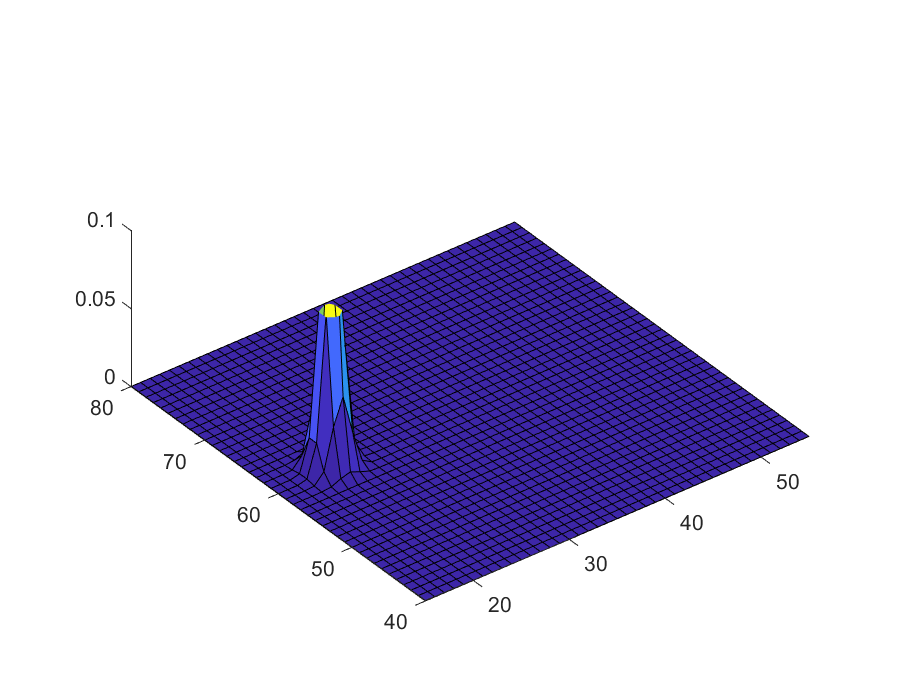
\includegraphics[width=\linewidth]{Figures/PDF_t0}
        \caption{t=0s}
        \label{fig:PDF_initial}
    \end{subfigure}%
    \begin{subfigure}{0.5\textwidth}
        \centering
        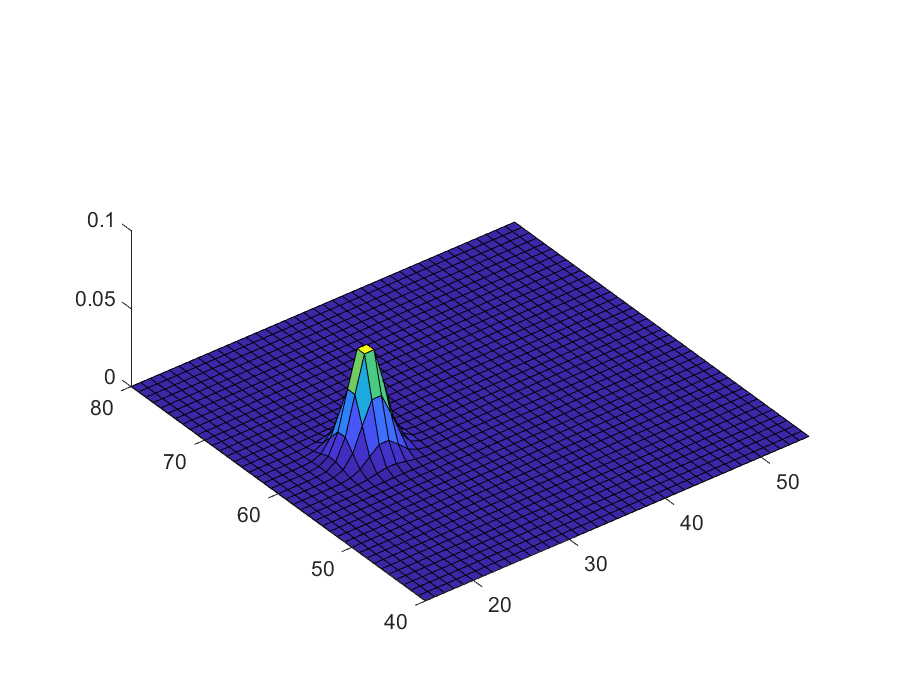
\includegraphics[width = \linewidth]{Figures/PDF_t5}
        \caption{t=5s}
        \label{fig:PDF_t5}
    \end{subfigure} \\
    \begin{subfigure}{.5\textwidth}
        \centering
    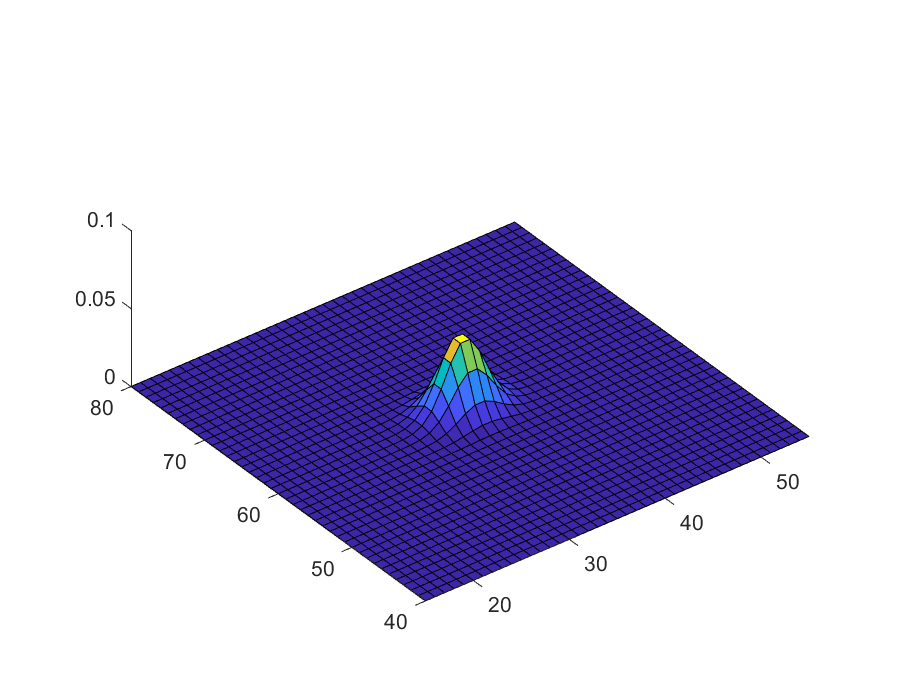
\includegraphics[width=\linewidth]{Figures/PDF_t15}
    \caption{t=15s}
    \label{fig:PDF_t15}
    \end{subfigure}%
    \begin{subfigure}{0.5\textwidth}
        \centering
    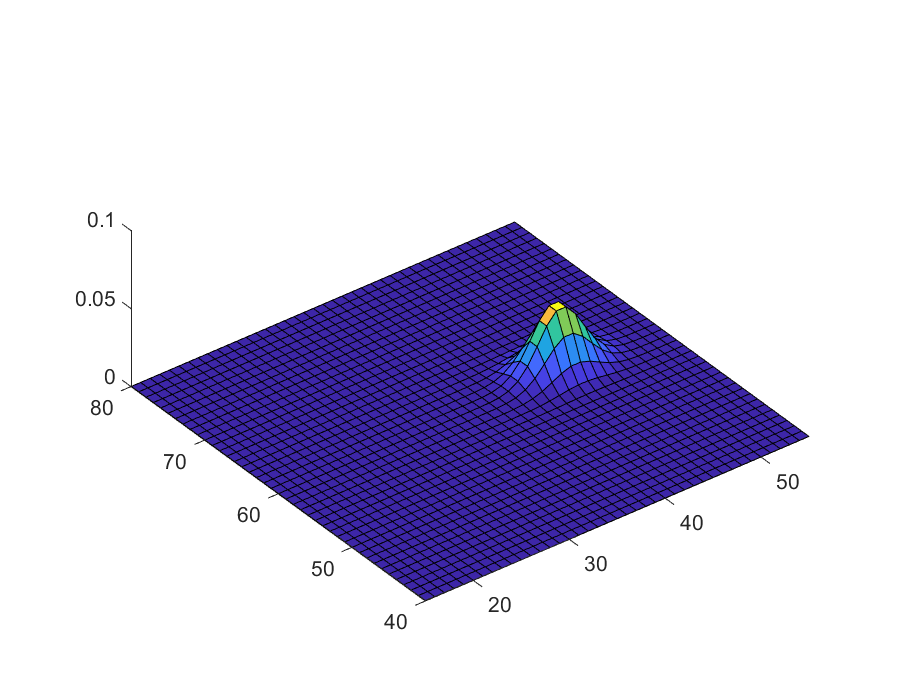
\includegraphics[width=\linewidth]{Figures/PDF_t20}
    \caption{t=20s}
    \label{fig:PDF_t20}
    \end{subfigure} 
    \caption{The probability density functions over the drone position at different time-steps in the simulation done by the MPC.}
    \label{fig:PDF_development}
\end{figure*}

\subsection{Varaince formulation}

To be able to propagate the variance through the system a linear system is required. The state space is linear, but the LOS guidance law is nonlinear due to the normalization of the $\chi^{NED}_{los,ca}$ vector in equation \eqref{V_ref,ca}. Nonlinearities will make a Gaussian curve loose its form making it difficult to propagate the system further.The system is linearized to compensate for this problem.

First the guidance law is re-written.

\begin{align}
    \chi^{NED}_{los,ca} & = R^{NED}_{los}  R_{ca} \left(  \begin{bmatrix}\Delta \\ 0 \\ 0\end{bmatrix} - \begin{bmatrix} 0 & 0 & 0 \\ 0 & 1 & 0 \\ 0 & 0 & 1 \end{bmatrix} R^{los}_{NED} (\begin{bmatrix} \mathbf{I} & \mathbf{0} \end{bmatrix} \hat{x} - WP_1) \right) \\
    & = E - F \hat{x}_p \\
     & = E - F x_p - F v_p \\
    E & = R^{NED}_{los}  R_{ca} \left(  \begin{bmatrix}\Delta \\ 0 \\ 0\end{bmatrix} + \begin{bmatrix} 0 & 0 & 0 \\ 0 & 1 & 0 \\ 0 & 0 & 1 \end{bmatrix} R^{los}_{NED} WP_1 \right) \\
    F & = R^{NED}_{los}  R_{ca}  \begin{bmatrix} 0 & 0 & 0 \\ 0 & 1 & 0 \\ 0 & 0 & 1 \end{bmatrix} R^{los}_{NED}\\
    x_p & = \begin{bmatrix}\mathbf{I}  &\mathbf{0}\end{bmatrix} x, \quad 
    \hat{x}_p  = \begin{bmatrix}\mathbf{I}& \mathbf{0}\end{bmatrix} \hat{x}, \quad
    v_p  = \begin{bmatrix}\mathbf{I}& \mathbf{0}\end{bmatrix} v 
\end{align}

Both x and v are stocastic variabels.$x$ contains the uncertainty in the state, $v$ describes the added uncertainty due to measurement errors. 

\begin{align}
        V_{ref,ca} & = v_0 \frac{\chi^{NED}_{los,ca} }{|| \chi^{NED}_{los,ca} ||} \\
        V_{ref,ca} & = v_0 \frac{E - F x_p - F v_p }{|| E - F x_p - F v_p ||}
\end{align}

This equation is linearized around the current expected $x$ value, $x=x_0$, and the expected value of the noise $v=v_0=0$. The expected $x$ value is calculated by the state space equation. The linearization is done in appendix A. This results in the following linearized equation

\begin{align}
        \bar{V}_{ref,ca}  ={}& v_0 (\bar{E} - \bar{F} x -\bar{F} v) \\
        \bar{E} ={}&  G + H \begin{bmatrix}\mathbf{I}  &\mathbf{0}\end{bmatrix} x_0 \\
        \bar{F} ={}& H \begin{bmatrix}\mathbf{I}  &\mathbf{0}\end{bmatrix} \\
        G ={}& \frac{E - F \begin{bmatrix}\mathbf{I}  &\mathbf{0}\end{bmatrix} x_0}{||E - F \begin{bmatrix}\mathbf{I}  &\mathbf{0}\end{bmatrix} x_0||} \\
        H ={}& \frac{F}{||E - F \begin{bmatrix}\mathbf{I}  &\mathbf{0}\end{bmatrix} x_0||}\\
                &-\left(\frac{(E - F \begin{bmatrix}\mathbf{I}  &\mathbf{0}\end{bmatrix} x_0)(E - F \begin{bmatrix}\mathbf{I}  &\mathbf{0}\end{bmatrix} x_0)^\top F}{||E - F \begin{bmatrix}\mathbf{I}  &\mathbf{0}\end{bmatrix} x_0||^3}\right)
\end{align}

Inserting the linearized velocity reference vector into the state space equation

\begin{align}
 x[k+1] & = A_{cl} x[k] + B_{cl} \bar{V}_{ref}[k] - \Gamma_{cl} v[k] +w_d[k] \\
 \bar{V}_{ref} & = v_0 (\bar{E} - \bar{F} x -\bar{F} v)
\end{align}

Resulting in
\begin{align}
 & x[k+1]   = A_{los} x[k] + \Gamma_{los} v[k] + w_d[k] + C_{los} \\ \label{linearized_los_eq}
 & A_{los}  = A_{cl} - B_{cl} v_0 \bar{F}, \quad \Gamma_{los} =  -\Gamma_{cl} - B_{cl} v_0 \bar{F})\\ & C_{los} = B_{cl} v_0 \bar{E}
\end{align}

We now have a linear state space formulation. With the asumption that $v[k]$ and $w[k]$ are white noise processes, all the terms in \eqref{linearized_los_eq} become uncorrelated and the covariance matrix of $x[k+1]$ can simply be calculated as

\begin{align}
    \textnormal{var}(x[k+1]) &= A_{los} \textnormal{var}(x[k]) A_{los}^\top + \Gamma \textnormal{var}(v[k]) \Gamma^\top + \textnormal{var}(w_d[k])  \\
    \textnormal{var}(x[k+1]) &= A_{los} \textnormal{var}(x[k]) A_{los}^\top + \Gamma R_d \Gamma^\top + Q_d
\end{align}

The initial variance is equal the position estimate variance, $R_d$. 
\begin{align}
    \textnormal{var}(x[0]) &= R_d
\end{align}

\subsection{Results}

%\begin{figure}[t]
    %\centering
    %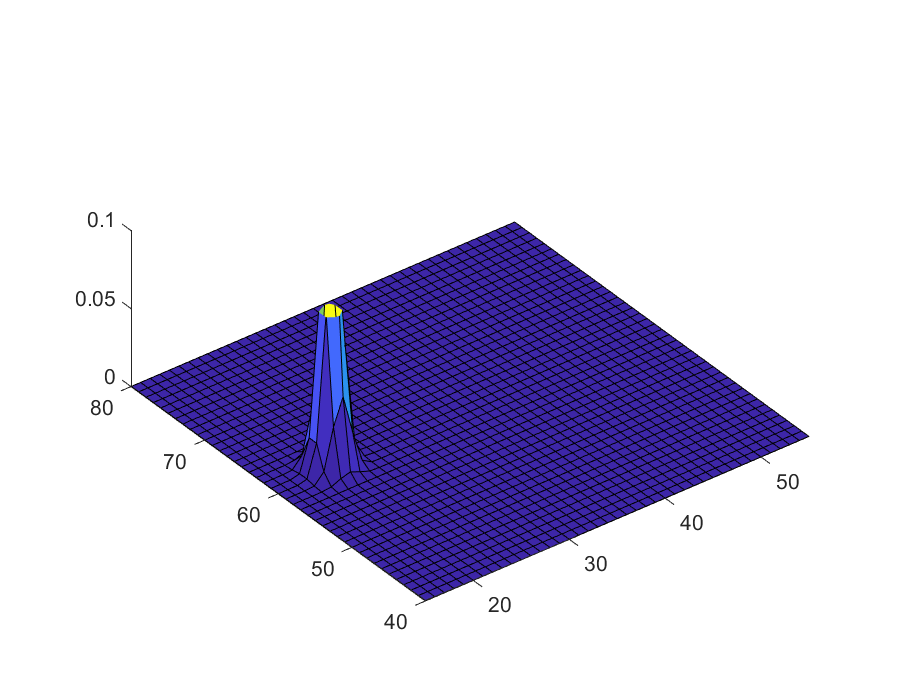
\includegraphics[width=\linewidth]{Figures/PDF_t0}
    %\caption{The initial probability density function of the drone position}
    %\label{fig:PDF_initial}
%\end{figure}

%\begin{figure}[t]
    %\centering
    %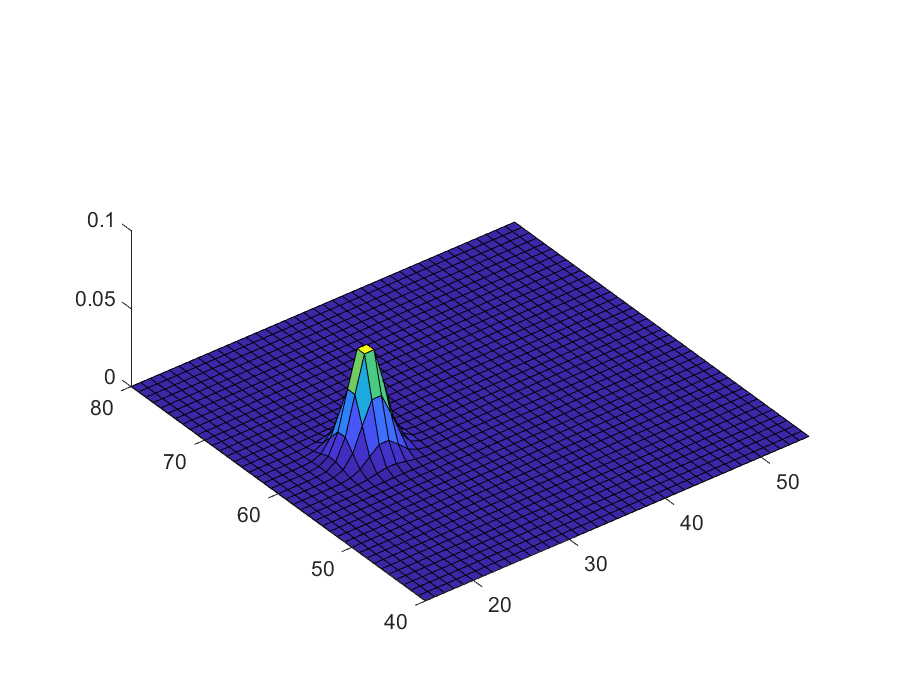
\includegraphics[width = \linewidth]{Figures/PDF_t5}
    %\caption{The probability density function of the drone position at t=5s}
    %\label{fig:PDF_t5}
%\end{figure}

%\begin{figure}[t]
    %\centering
    %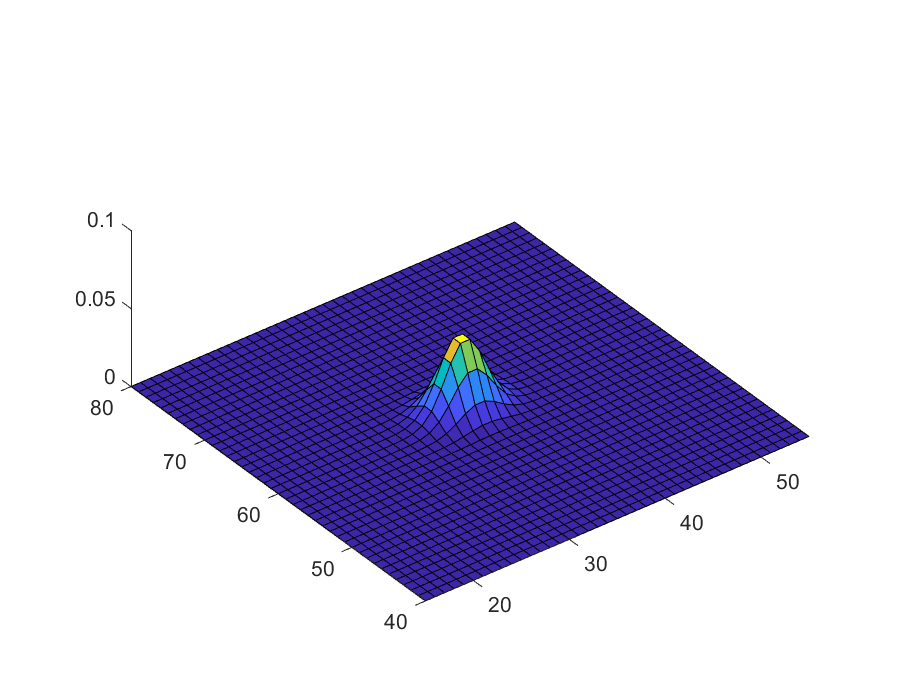
\includegraphics[width=\linewidth]{Figures/PDF_t15}
    %\caption{The probability density function of the drone position at t=15s}
    %\label{fig:PDF_t15}
%\end{figure}

%\begin{figure}[t]
    %\centering
    %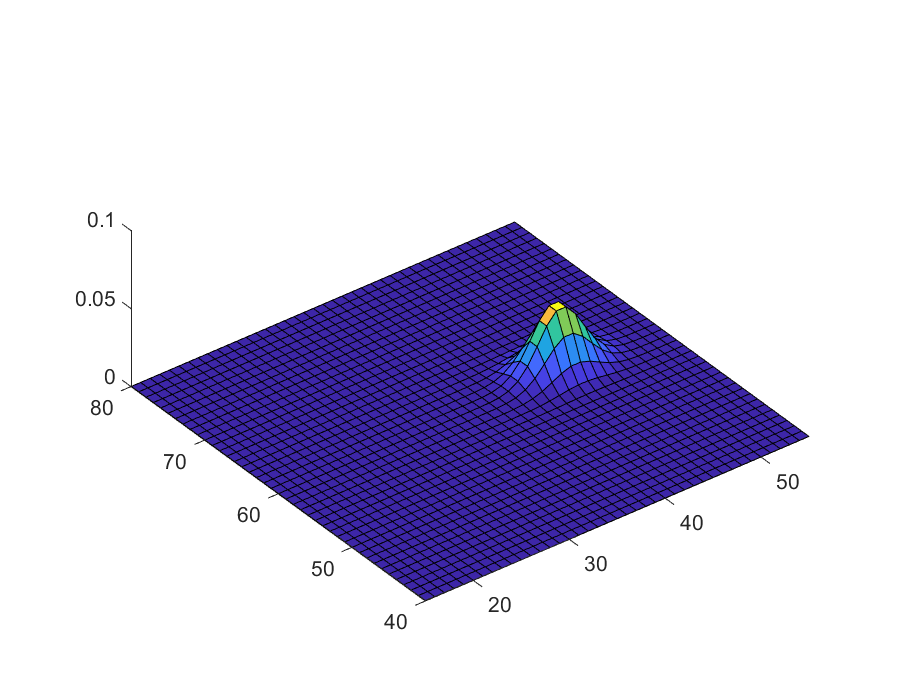
\includegraphics[width=\linewidth]{Figures/PDF_t20}
    %\caption{The probability density function of the drone position at t=20s}
    %\label{fig:PDF_t20}
%\end{figure}

The uncertainty in position will start low as and then gradually increase as seen in figure \ref{fig:PDF_development}. Its interesting to note that the probability density function becomes elongated over time, the uncertainty is larger in the along path direction than in the across path direction. This is a direct consequence of LOS guidance being asymptotically stable in across path direction, but only marginally stable in the along path direction, since the LOS guidance law does not try to counteract along path errors.
\section{Sensor model}
\subsection{Radar sensor}
In this work a simple radar model is used. The radar is assumed to be able to detect things within a cone with a given spread and maximum range. The radar will give out the distance to the nearest object that overlaps the cone. Where inside the cone the object is, is unknown, only the distance to the object and the fact that the object is inside the cone is known. Figure \ref{fig:SensorData} shows the data gathered from 5 radar sensors. Black indicates that there is an obstacle that reflected the radar beam at that distance. White is safe areas where no obstacle has been detected. Gray is areas with no information. The radar beams are here made thinner to be able to distinguish them in the figure. In the rest of this paper, the radars will be made thicker such that the gap between them is removed. Figure \ref{fig:SuperimposedSensorData} shown where the obstacles really are. Determining the shape and location of the obstacles based on figure \ref{fig:SensorData} alone is impossible. Instead sensor data over time has to be combined.

\begin{figure}[!t]
\begin{subfigure}[b]{0.48\linewidth}
    \centering
    
\includegraphics[width= 1.2\linewidth]{Figures/radar_data.eps}
    \caption{}
    \label{fig:SensorData}
\end{subfigure}
\begin{subfigure}[b]{0.48\linewidth}
    \centering
    
\includegraphics[width= 1.2\linewidth]{Figures/radar_data_superimposed.eps}
    \caption{}
    \label{fig:SuperimposedSensorData}
\end{subfigure}
\caption{Representation of the sensor-data from the stationary radar sensors. \ref{fig:SuperimposedSensorData} shows the sensordata superimposed on the true obstacle map }
\end{figure}


A grid-map is used to save the radar data over time. Each grid holds the probability of there being an object in that grid. The probabilities are simplified to only having three values,  1 if we have measured that there might be something in that grid, 0.5 if we have not measured the spot, and 0 if we know that the spot is safe. When a radar measurement is made, then all grids within the cone closer to the drone than the measured distance to the closest obstacle are marked as safe with a value 0. All cells further away than the measured distance that are within some penetration depth are assumed to contain an obstacle. These cells are marked as dangerous, 1, if they were previously marked as unknown. Since the radar may mark too many cells as potentially dangerous, the measurement of safe cells should trump a marked potentially dangerous cell. This way the drone will start with a restrictive map where too many cells are marked as dangerous, and after more measurements with different angles the safe cells will gradually be marked as safe.  Figure \ref{fig:Combined_obstacle_map} shows how the map can end up looking after the drone has flown along some route. 

\begin{figure}[!t]
\begin{subfigure}[b]{0.48\linewidth}
    \centering
    
\includegraphics[width= 1.2\linewidth]{Figures/radar_after_flying}
    \caption{}
    \label{fig:Combined_obstacle_map}
\end{subfigure}
\begin{subfigure}[b]{0.48\linewidth}
    \centering
    
\includegraphics[width= 1.2\linewidth]{Figures/radar_after_flying_superimposed}
    \caption{}
\end{subfigure}
\caption{The obstacle map after flying along the marked path.  }
\end{figure}

The penetration depth should be designed large enough such that if the drone probability density function moves through it, then 95\% of Gaussian position curve should be inside the area marked as dangerous at some point. $\pm2 \sigma_p$, where $\sigma_p$ is the largest uncertainty in position over the time horizon, will encompass 95\% of the Gaussian curve that marks the uncertainty in position. In addition a margin has to be added due to the discrete time-steps to ensure that there exists a time-step when the curve is inside the marked area. The penetration depth should then be chosen as follows.
    \begin{equation}
        d_p = 4\sigma_p +dt v_0 \label{penetration_deapth}
    \end{equation}


This strategy for combining sensor data will not work in reality as it is not robust against measurement or position estimate errors. The cells should also give some sort of probability that there is an obstacle in the cell, and not the clean cut 0, 0.5, 1 probabilities it does now. The radar sensor model and combining of data requires further work. 
\section{Scenario based MPC formulation}
\subsection{Constraint}
Forklar tidshorisonten
        HVrodan drone prob og verden prob slåes sammen
        HVordan usikkerhet over tid slås sammen

\subsection{Objective}
        Hvordan along path offset beregnes
        Datatap? Integral av feil avstand?
        
\subsection{Default action}
når det er infeasable
        Forklar at om vi er i ett utrygt punkt burde vi heller pelle oss vekk enn å bli
        Ellers stopp
\section{Parameter choices}
\section{Results}
 Dronen som klarer at veggen er oppå planne path
    Hindring i veien for planned path
    Kjører rolig rundt hjørner /større sirkel for å få data før den går inn i faresonen
    Takler problemfritt at det er en ukjent hindring rett rundt hjørnet
    
    Feiler:
        Blir stuck i konvekse hull
        Blir stuck i ting som er konvekse hull men ikke ser sånn ut siden wp snur seg.
\section{Conclusion}

This work has developed a control strategy for collision avoidance in an unknown environment that guarantees an acceptable risk level. The method includes uncertainty's in predicted position from imperfect control inputs based on noisy measurements, as well as direct disturbance affecting the drone. Simple 2D simulations suggests that this control strategy manages to successfully avoid collision within the given risk level, with simple radar sensors as the perception sensors. The control strategy leads to safe behaviour such as not flying blindly around a corner, and instead flying in a larger circle to gather more data. But as the strategy is a greedy, it is unable to avoid getting stuck in convex hulls. Even though it is not able to avoid getting stuck, it will avoid collision, and instead stop or fly slowly back and forth. A higher level controller that designes the waypoints, can then detect that the drone is stuck and re-plan the waypoints around the convex area.

The developed strategy is quite computationally simple with a short time horizon and few possible control actions that must be simulated. Almost all control actions can be simulated separately before comparison, which opens up for parallel computing. Whether this simplicity leads to fast computations is not yet determined, and depends a lot on how quick the probability density function of the drone can be computed. 

The developed strategy requires no tuning of parameters that significantly affect the performance. A strategy for choosing all parameters that require asigning is presented for all but the process noise Q. 


\section{Future work}

Before this algorithm can be tested in practice the drone model has to be developed into a 3D model with attitude dynamics. Including attitude might significantly affect how the positional variance develops over time. Furthermore a new robust strategy for combining sensor data has to be developed, this strategy should encompass how reliably the information is. The physical size of the drone has to be included. This can be done by diluting the obstacle map with an ellipsoid with the same general dimensions as the drone. Lastly a strategy for calculating probability of collision over a time horizon has to be developed. The probability that the drone will collide over the time-horizon is the constraint we really care about. 


%Estimating the size of the process disturbance is  

%Velge tryggere veier



%%%%%%%%%%%%%%%%%%%%%%%%%%%%%%%%%%%%



%%%%%%%%%%%%%%%%%%%%%%%%%%%%%%%%%%%%%%%%%%%%%%%%%%%%%%%%%%%%%%%%%%%%%%%%%%%%%%%%
\section*{APPENDIX}

\section*{ACKNOWLEDGMENT}



\end{document}
